Let's train a neural network to classify these digits, using 60,000 input/output examples in \texttt{trainData} dataset for supervised learning and evaluate the performance on 10,000 examples in the \texttt{testData} dataset.

\subsection{Choosing the network architecture}
It would be a good idea to use some well-known architecture that was trained on other platforms. This way we can easily compare the performance. Here are the two architectures I will be working with in this chapter
\begin{enumerate}
  \item Single-layer neural network with $784$ inputs and $10$ neurons. All neurons have softmax activation function. The learning rate is constant and set to $0.5$. The network uses Cross-entropy cost function
\end{enumerate}

\newcommand{\net1}{Experiment 1}
\newcommand{\net2}{Experiment 2}

\begin{table}[h!]
  \renewcommand\arraystretch{1.2}
  \centering
  
  \begin{tabularx}{0.75\textwidth}{|H|CC|}
    \hline
                    & \net1             & \net2 \\
    \hline
    Architecture    & 784, 10           & 784, 500, 10       \\
    Activations     & Softmax           & Logistic, Softmax \\
    Cost            & Cross-entropy     & Cross-entropy \\
    \hline
  \end{tabularx}
  
  \caption{Table to test captions and labels}
  \label{table:architectures}
\end{table}

\begin{table}[h!]
  \renewcommand\arraystretch{1.2}
  \centering
  
  \begin{tabularx}{0.75\textwidth}{|H|CC|}
    \hline
                    & \net1             & \net2 \\
    \hline
    Batch size      & 100               & 100 \\
    Epochs          & 1000              & 500 \\
    Learning rate   & 0.5               & 0.1 \\
    \hline
  \end{tabularx}
  
  \caption{Table to test captions and labels}
  \label{table:training}
\end{table}

The results obtained after training

\begin{table}[h!]
  \renewcommand\arraystretch{1.2}
  \centering
  
  \begin{tabularx}{0.75\textwidth}{|H|CC|}
    \hline
                    & \net1             & \net2 \\
    \hline
    Accuracy        & 92\%              & 88\% \\
    Training time   & 0:00:07:02.85     & 0:06:15:31.29 \\
    Time per epoch  & 0:00:00:00.42     & 0:00:00:45.06 \\
    \hline
  \end{tabularx}
  
  \caption{Table to test captions and labels}
  \label{table:results}
\end{table}

\subsection{Single-layer neural network (784, 10)}

\begin{lstlisting}
neuralNet := MLNeuralNetwork new initialize: #(784 10).
neuralNet outputLayer activationFunction: (MLSoftmax new).
neuralNet costFunction: (MLCrossEntropy new).
neuralNet lerningRate: 0.5.

neuralNet learningAlgorithm: (MLMiniBatchBackpropagation new).
neuralNet batchSize: 100.
\end{lstlisting}

\begin{lstlisting}
neuralNet learn: trainingData epochs: 1000.
\end{lstlisting}

\begin{figure}[H]
  \centering
  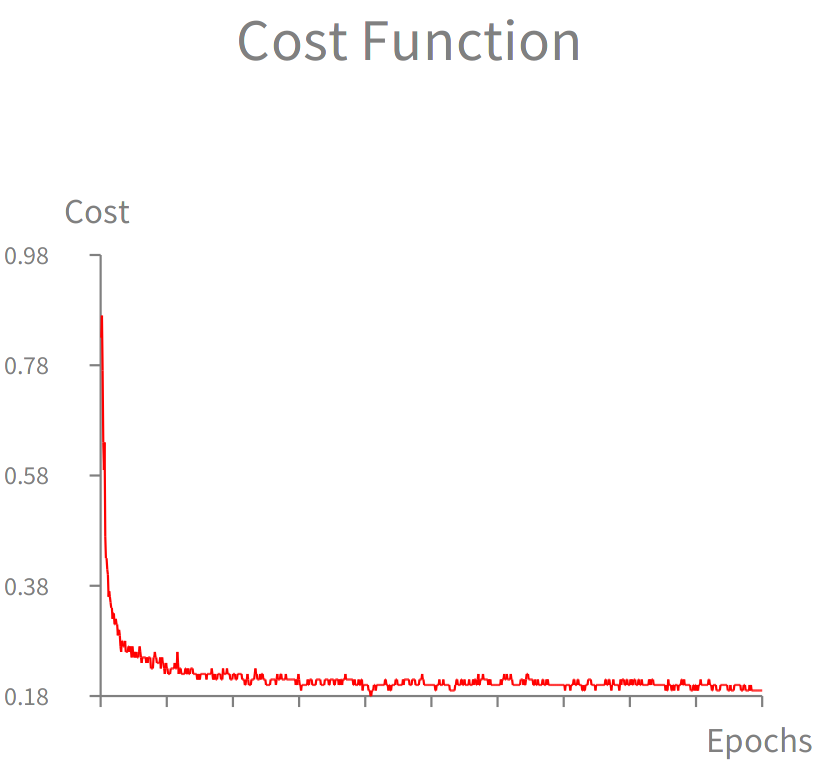
\includegraphics[width=\imgwidth]{cost-784-10}
  \caption{Cost history of a single-layer neural network}
  \label{fig:cost-784-10}
\end{figure}

\subsection{Two-layer neural network (784, 500, 10)}

\begin{lstlisting}
neuralNet := MLNeuralNetwork new initialize: #(784 500 10).
(neuralNet layerAt: 1)
neuralNet outputLayer activationFunction: (MLSoftmax new).
neuralNet costFunction: (MLCrossEntropy new).
neuralNet lerningRate: 0.5.

neuralNet learningAlgorithm: (MLMiniBatchBackpropagation new).
neuralNet batchSize: 100.
\end{lstlisting}

\begin{lstlisting}
neuralNet learn: trainingData epochs: 1000.
\end{lstlisting}

\begin{figure}[H]
  \centering
  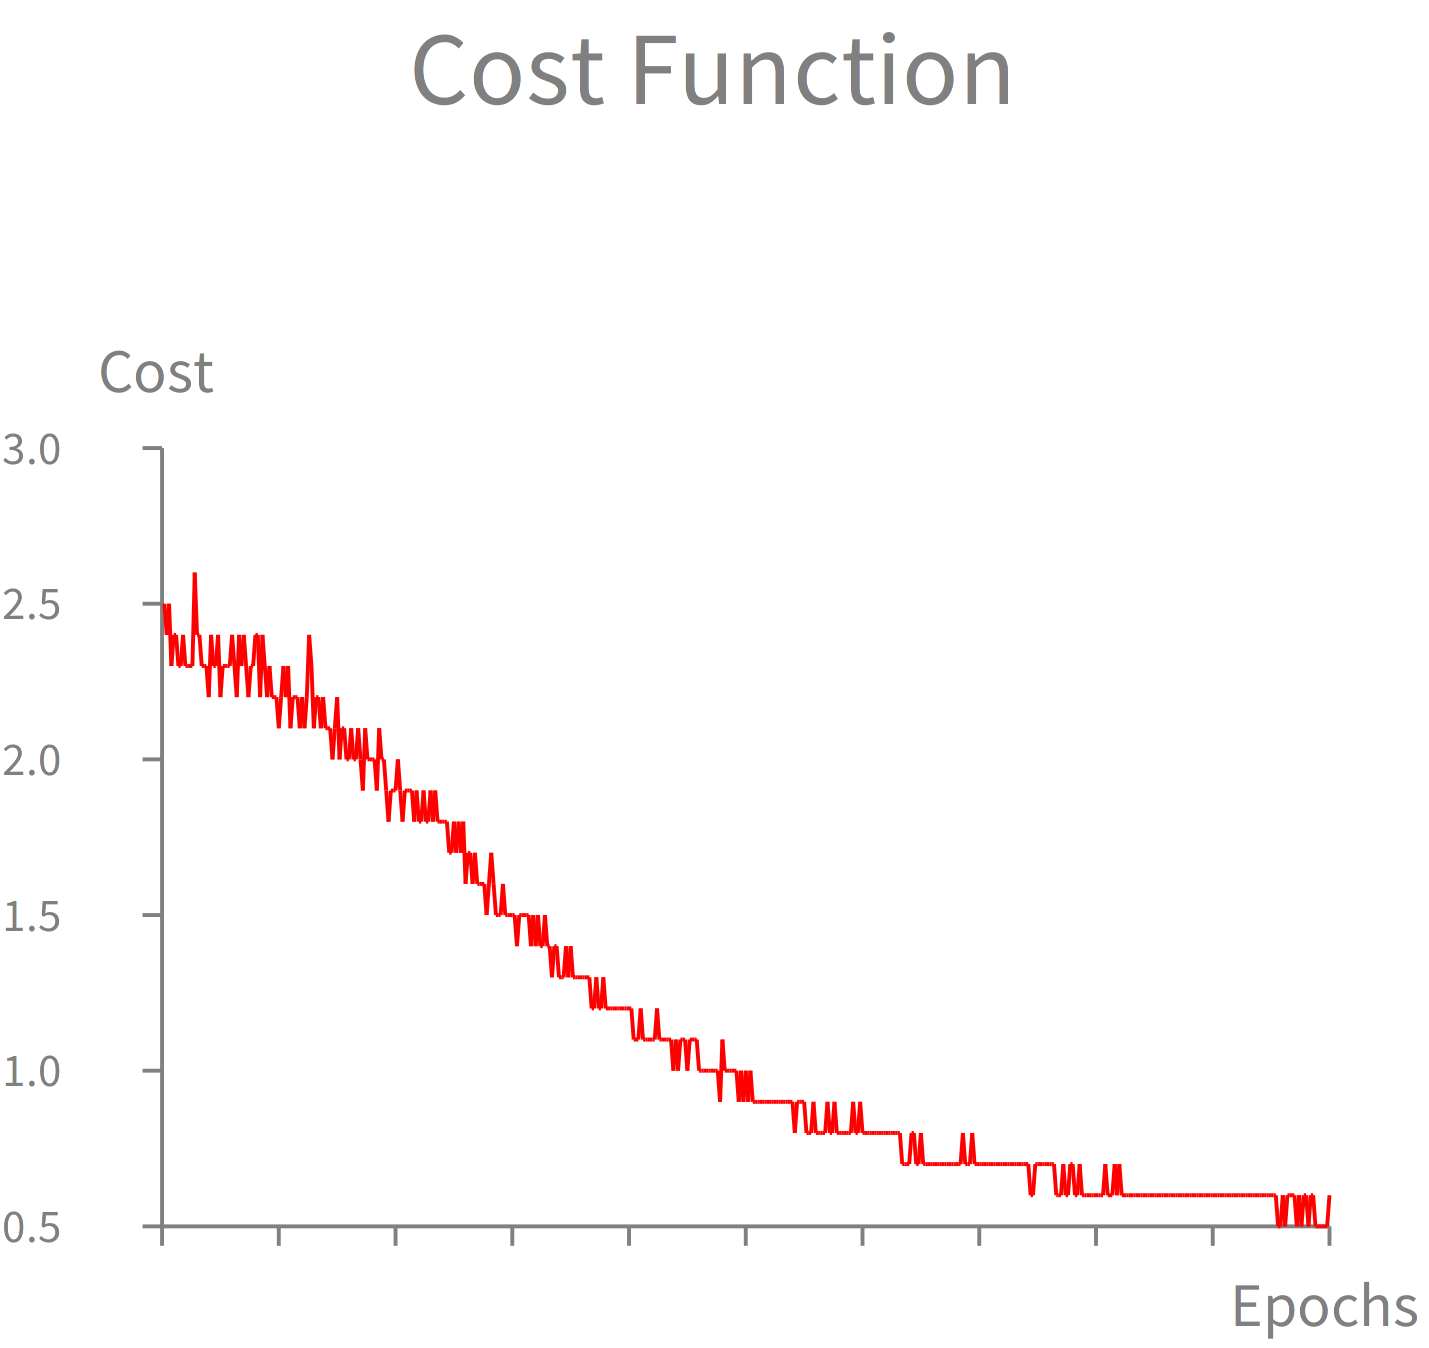
\includegraphics[width=\imgwidth]{cost-500-01}
  \caption{Cost history of a two-layer neural network with 500 hidden units. The network was trained with mini-batches of size 100 during 500 epochs and with learning rate 0.1 }
  \label{fig:cost-500-01}
\end{figure}

The Roassal\cite{Bergel} visualization of a random prediction made by a trained neural network with softmax output layer. The activity of 10 output neurons is probabilistic and sums up to 1. The neuron with the highest activity indicates the prdicted class. The bar of a correct (expected) class is green. If you see only one colorful bar, it means that the network made a correct prediction. If the network made a mistake and the highest bar is different from the targeted class, it is highlited in red. Then you can see a green bar indicating the correct class, and the red bar of the class that was incorrectly predicted.

\begin{figure}[H]
  \centering
  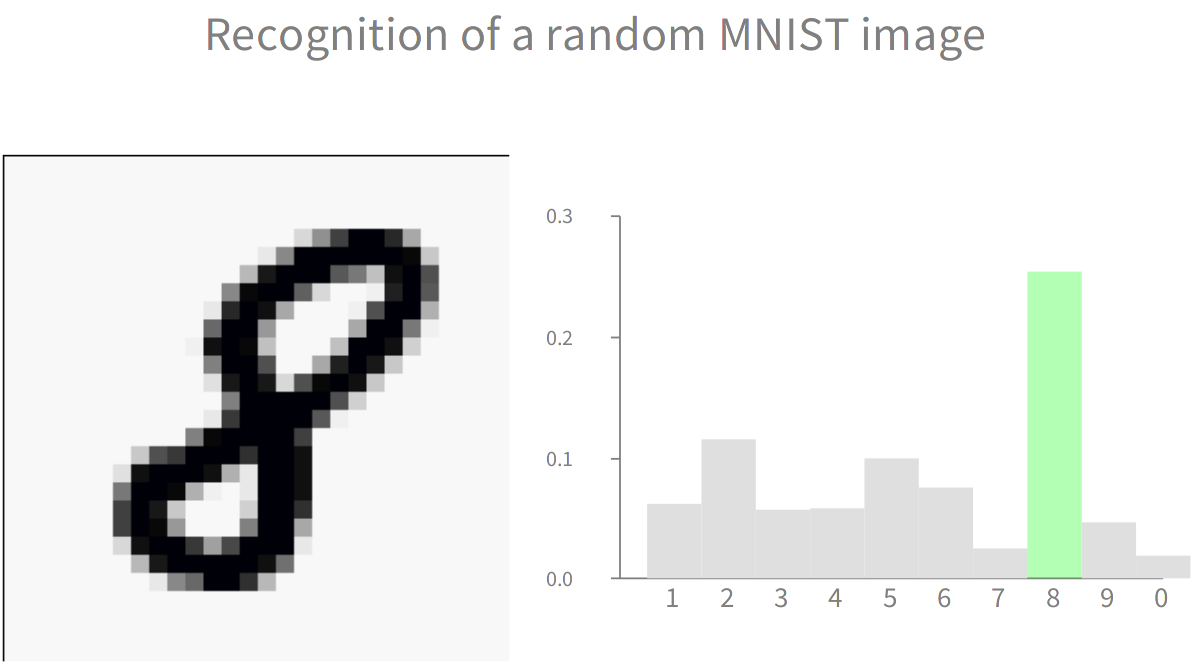
\includegraphics[width=\imgwidth]{pred8}
  \caption{Predicting random MNIST image}
  \label{fig:pred8}
\end{figure}
